\section{Starter-Monster}\label{sec:starter-monster}
Der Erhalt von Monstern wird dem Nutzer anfänglich erleichtert.
In diesem Release wird der Erhalt des Starter-Monsters von dem NPC-Trainer Prof. Albert bereitgestellt, wenn der Nutzer mit ihm einen Dialog startet und eine Auswahl an Monstern trifft.
\subsection{Mockups}\label{subsec:mockups-starter-monster}
Der Nutzer steht in der Abbildung~\ref{fig: User and Prof. Albert voreinander} vor dem NPC-Trainer Prof. Albert und startet einen Dialog nach dem Drücken der Interaktionstaste.
In diesem Dialog wie in Abbildung~\ref{fig: Dialog Nutzer und Prof. Albert} heißt der NPC-Trainer Prof. Albert den Nutzer willkommen und bietet ihm verschiedene Starter-Monster an.
Diese Starter-Monster sieht der Nutzer ebenfalls nach Drücken der Interaktionstaste.  
\begin{figure}[H]
    \centering
    \begin{subfigure}[b]{0.4\textwidth}
        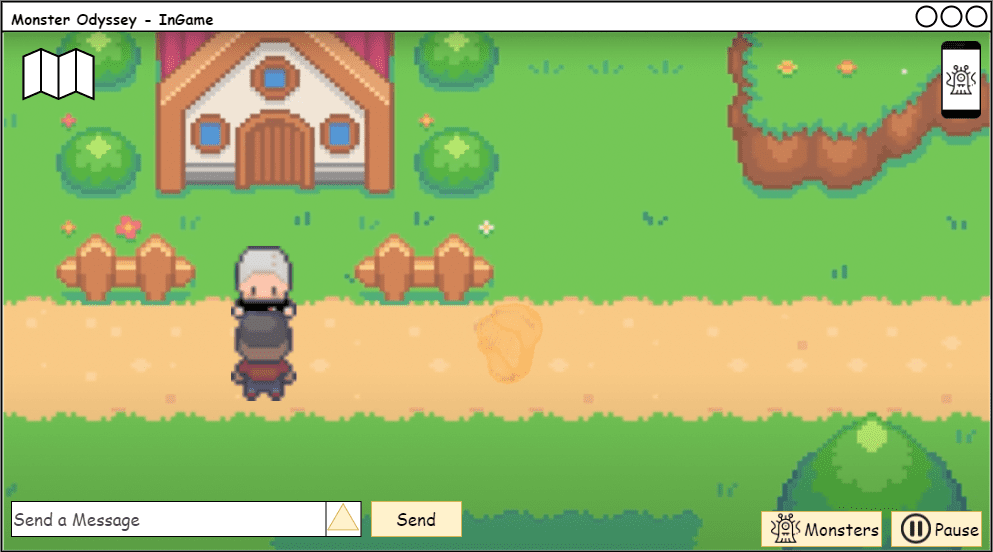
\includegraphics[width=\textwidth]{images/mockups/Starter/PlayerAndProf}
        \caption{Nutzer und Prof. Albert voreinander}
        \label{fig: User and Prof. Albert voreinander}
    \end{subfigure}
    \hfill
    \begin{subfigure}[b]{0.4\textwidth}
        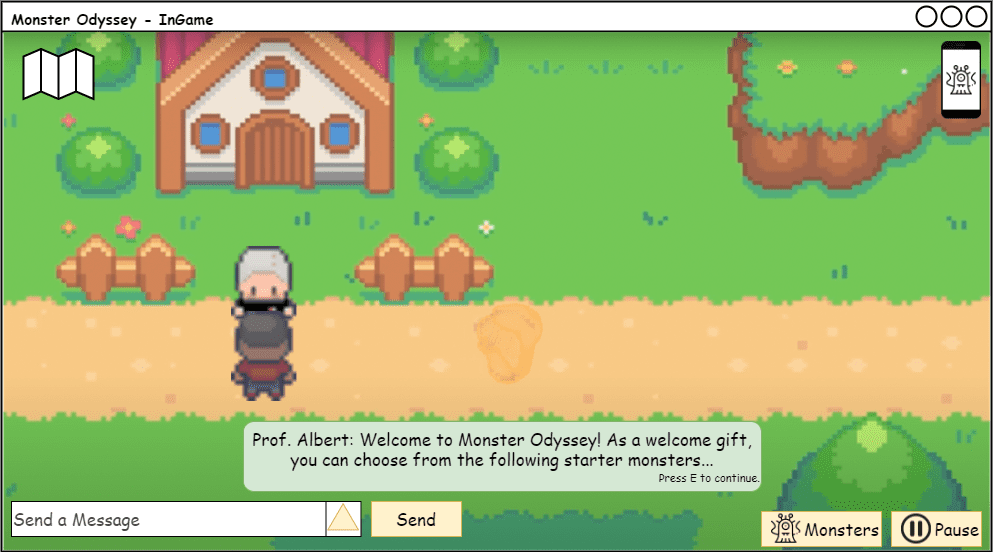
\includegraphics[width=\textwidth]{images/mockups/Starter/PlayerAndProfMessage}
        \caption{Dialog zwischen Nutzer und Prof. Albert}
        \label{fig: Dialog Nutzer und Prof. Albert}
    \end{subfigure}
    \caption{Mockup: Starten eines Dialogs mit Prof. Albert}
    \label{fig: Starten eines Dialogs mit Prof. Albert}
\end{figure}
Nachdem der Nutzer die Interaktionstaste getätigt hat, erscheint ein Popup wie in Abbildung~\ref{fig: Erste Auswahl an Starter-Monstern}, indem die Selektion des Starter-Monsters stattfindet.
Es werden drei verschiedene Monster angeboten, die von dem Server festgelegt sind.
Im Folgenden werden die Elemente nur anhand der ersten Auswahl an Starter-Monstern beschrieben.
In diesem Popup sind ein Bild, ein Monster-Typ, ein Name und eine kurze Beschreibung des jeweiligen Monsters dargestellt. Der Monster-Typ ist in einem Kästchen platziert, das farblich nach diesem Typen gekennzeichnet ist. Diese dargelegten Elemente variieren je nach dem aktuell ausgewählten Monster.
Durch die Pfeile auf der linken beziehungsweise rechten Seite des Popups kann der Nutzer zunächst zum angebotenen Starter-Monster wechseln und seine zugehörigen Elemente sehen.
\begin{figure}[H]
    \center
    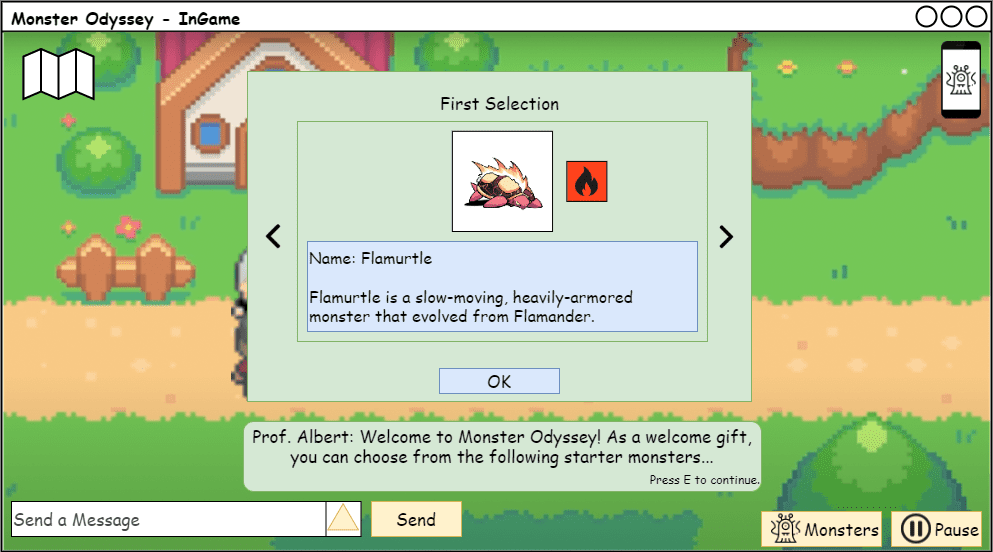
\includegraphics[scale=\scale]{images/mockups/Starter/PlayerAndProfMonsterSelection}
    \caption{Mockup: Erste Auswahl an Starter-Monstern}
    \label{fig: Erste Auswahl an Starter-Monstern}
\end{figure}
Entscheidet sich der Nutzer für ein Starter-Monster, so kann er mit dem 'OK'-Knopf auf dem Popup aus Abbildung~\ref{fig: Erste Auswahl an Starter-Monstern} seine Auswahl bestätigen.  Somit erhält der Nutzer das ausgewählte Starter-Monster und dieses wird zu der Monsterliste des Nutzers hinzugefügt. Dabei erscheint erneut ein Popup, wie in Abbildung~\ref{fig: Erhaltener Starter-Monster}, mit den Elementen des Monsters, zusätzlich erscheint eine Beschriftung, dass das Monster hinzugefügt wurde.
Beim Drücken des 'OK'-Knopfs wird der Dialog fortgesetzt, in dem der NPC-Trainer Prof. Albert dem Nutzer viel Erfolg wünscht. Der Dialog kann beendet werden, wenn der Nutzer in der Spielsituation wie in der Abbildung~\ref{fig: Nach Erhalt des Starter-Monsters} die Interaktionstaste tätigt.
\begin{figure}[H]
    \center
    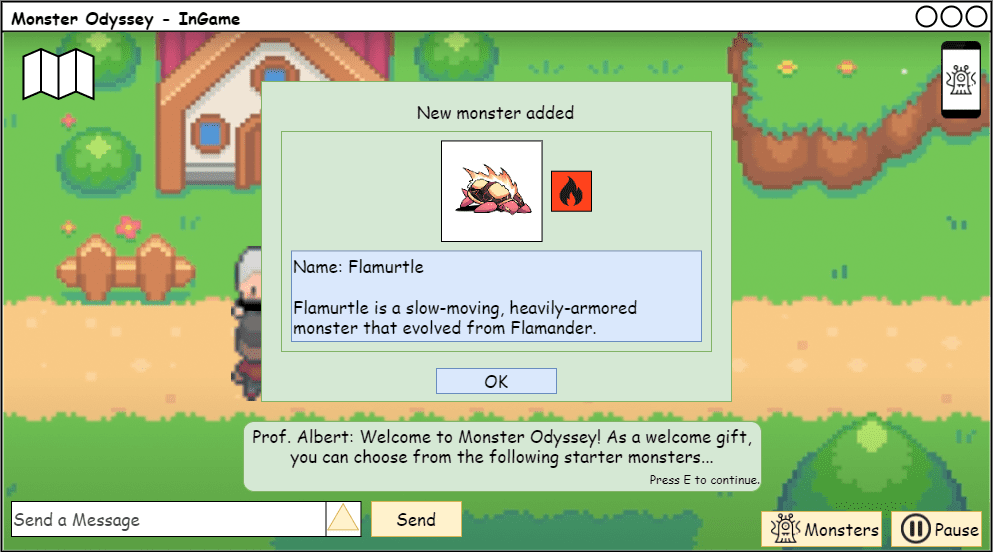
\includegraphics[scale=\scale]{images/mockups/Starter/PlayerAndProfMonsterReceived}
    \caption{Mockup: Erhaltener Starter-Monster}
    \label{fig: Erhaltener Starter-Monster}
\end{figure}
\begin{figure}[H]
    \center
    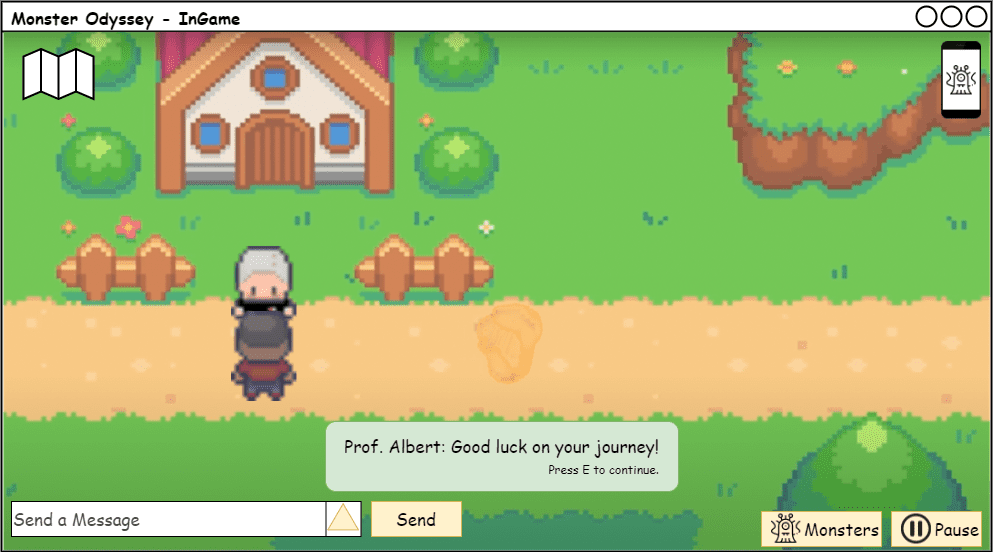
\includegraphics[scale=\scale]{images/mockups/Starter/PlayerAndProfAfterReceived}
    \caption{Mockup: Nach Erhalt des Starter-Monsters}
    \label{fig: Nach Erhalt des Starter-Monsters}
\end{figure}
Falls der Nutzer bereits ein Starter-Monster von dem NPC-Trainer Prof. Albert erhalten hat, so wird der Nutzer beim Interagieren mit ihm einen Dialog starten, aber keine neuen Starter-Monster bekommen können. Dabei weist Prof. Albert den Nutzer wie in Abbildung~\ref{fig: Starter-Monster bereits erhalten} darauf hin, dass er bereits dem Nutzer ein Starter-Monster überreicht hatte.
\begin{figure}[H]
    \center
    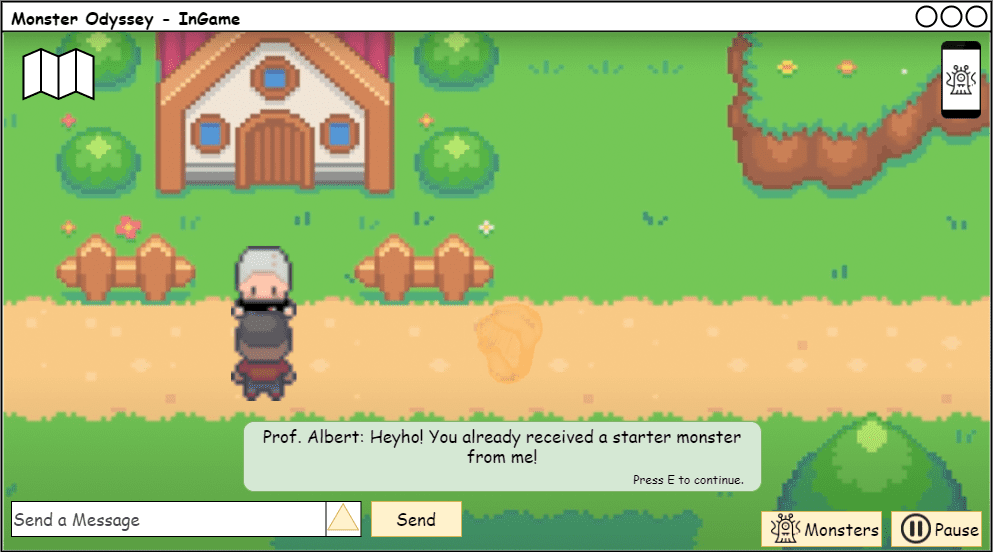
\includegraphics[scale=\scale]{images/mockups/Starter/PlayerAndProfAlreadyReceived}
    \caption{Mockup: Starter-Monster bereits erhalten}
    \label{fig: Starter-Monster bereits erhalten}
\end{figure}
\subsection{Vergleich zwischen Mockups und Implementierung}\label{subsec:vergleich-zwischen-mockups-und-implementierung-starter-monster}
In der Abbildung~\ref{fig: Vergleich: Starten eines Dialogs mit Prof. Albert} sind die Elemente des Dialogsystems verschieden, was in Abschnitt~\ref{subsec:vergleich-zwischen-mockups-und-implementierung-dialogsystem} angedeutet wurde. Auch die Dialogtexte variieren, um in der Implementierung ansprechendere und humoristische Dialogtexte zu formulieren, damit das Spielerlebnis unterhaltsam gestaltet wird.
\begin{figure}[H]
    \centering
    \begin{subfigure}[b]{0.4\textwidth}
        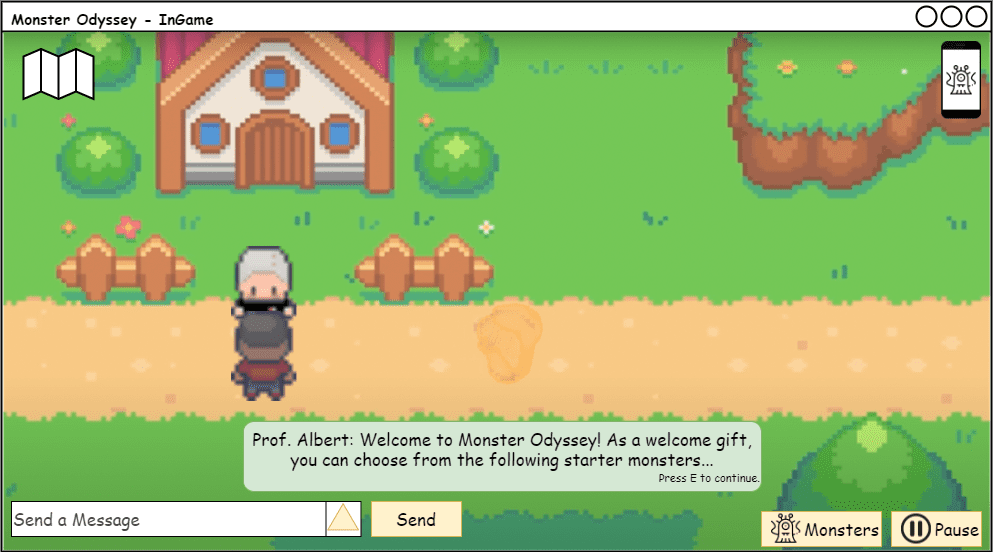
\includegraphics[width=\textwidth]{images/mockups/Starter/PlayerAndProfMessage}
        \caption{Mockup: Dialog zwischen Nutzer und Prof. Albert}
        \label{fig: Mockup: Dialog Nutzer und Prof. Albert}
    \end{subfigure}
    \hfill
    \begin{subfigure}[b]{0.4\textwidth}
        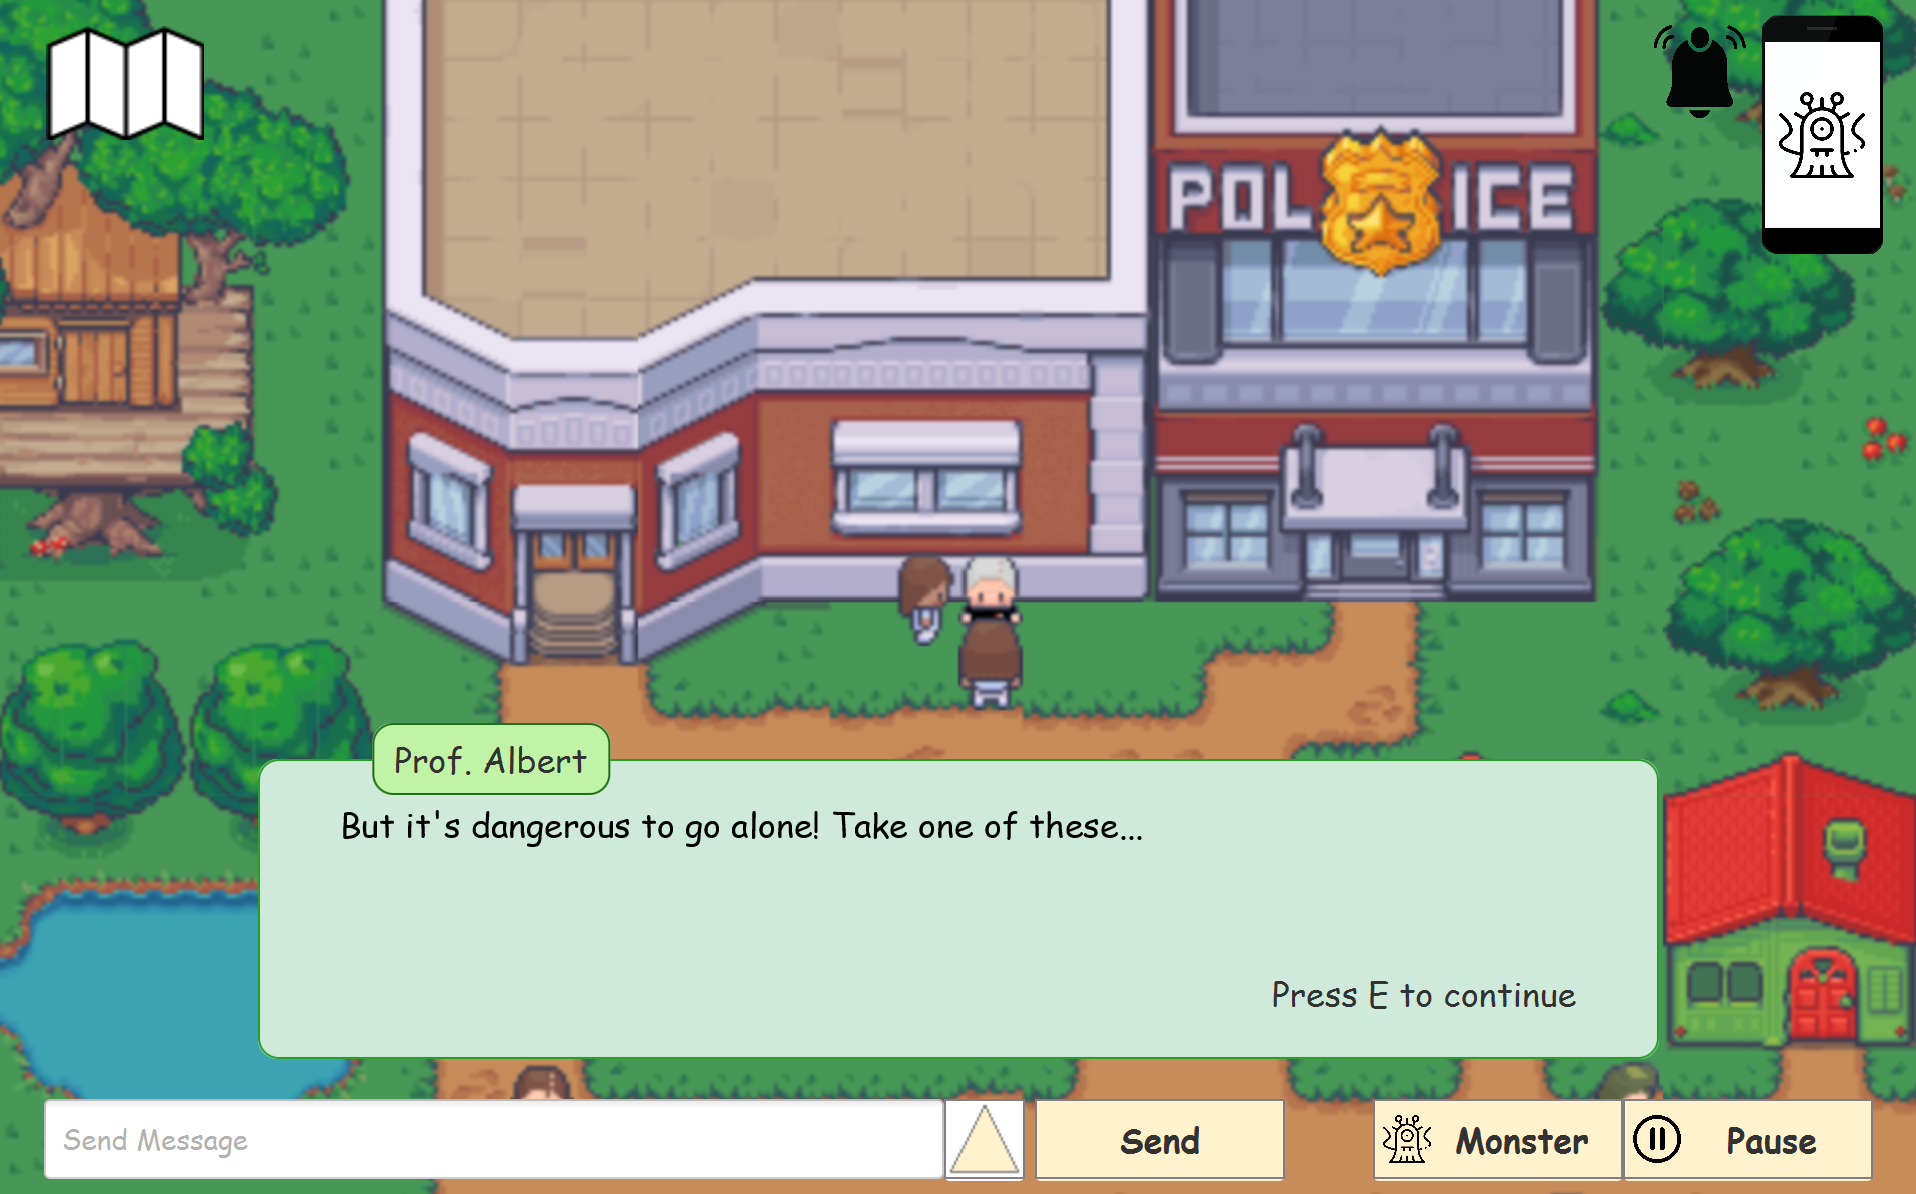
\includegraphics[width=\textwidth]{images/implementation/Starter/Implement dialog.png}
        \caption{Implementierung: Dialog zwischen Nutzer und Prof. Albert}
        \label{fig: Implementierung: Dialog Nutzer und Prof. Albert}
    \end{subfigure}
    \caption{Vergleich: Starten eines Dialogs mit Prof. Albert}
    \label{fig: Vergleich: Starten eines Dialogs mit Prof. Albert}
\end{figure}
Darüber hinaus ist in der Abbildung~\ref{fig: Vergleich: Auswahl an Starter-Monsters} zu sehen, dass die Elemente in den Mockups mit den Elementen in der Implementierung identisch sind, wobei die Starter-Monster verschieden sind. Der Hintergrund erhält einen Unschärfeeffekt, um dadurch die Konzentration des Nutzers auf die Auswahl an Starter-Monster zu lenken.

In der Abbildung~\ref{fig: Vergleich: Erhaltener Starter-Monster} ist zu bemerken, dass die Elemente, abgesehen von den Unterschieden aus den vorherigen Abbildungen, übereinstimmend sind. 
\begin{figure}[H]
    \centering
    \begin{subfigure}[b]{0.4\textwidth}
        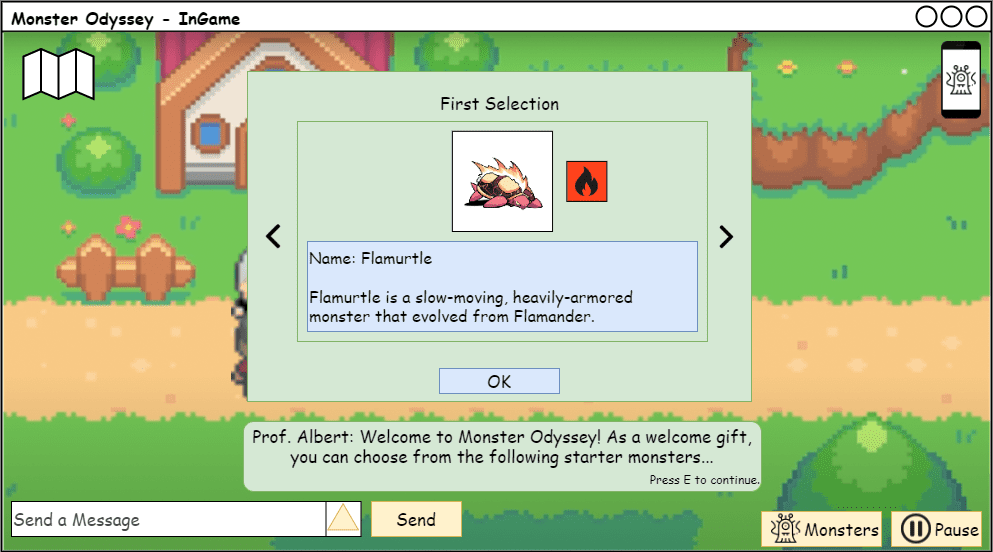
\includegraphics[width=\textwidth]{images/mockups/Starter/PlayerAndProfMonsterSelection}
        \caption{Mockup: Erste Auswahl an Starter-Monstern}
        \label{fig: Mockup: Erste Auswahl an Starter-Monstern}
    \end{subfigure}
    \hfill
    \begin{subfigure}[b]{0.4\textwidth}
        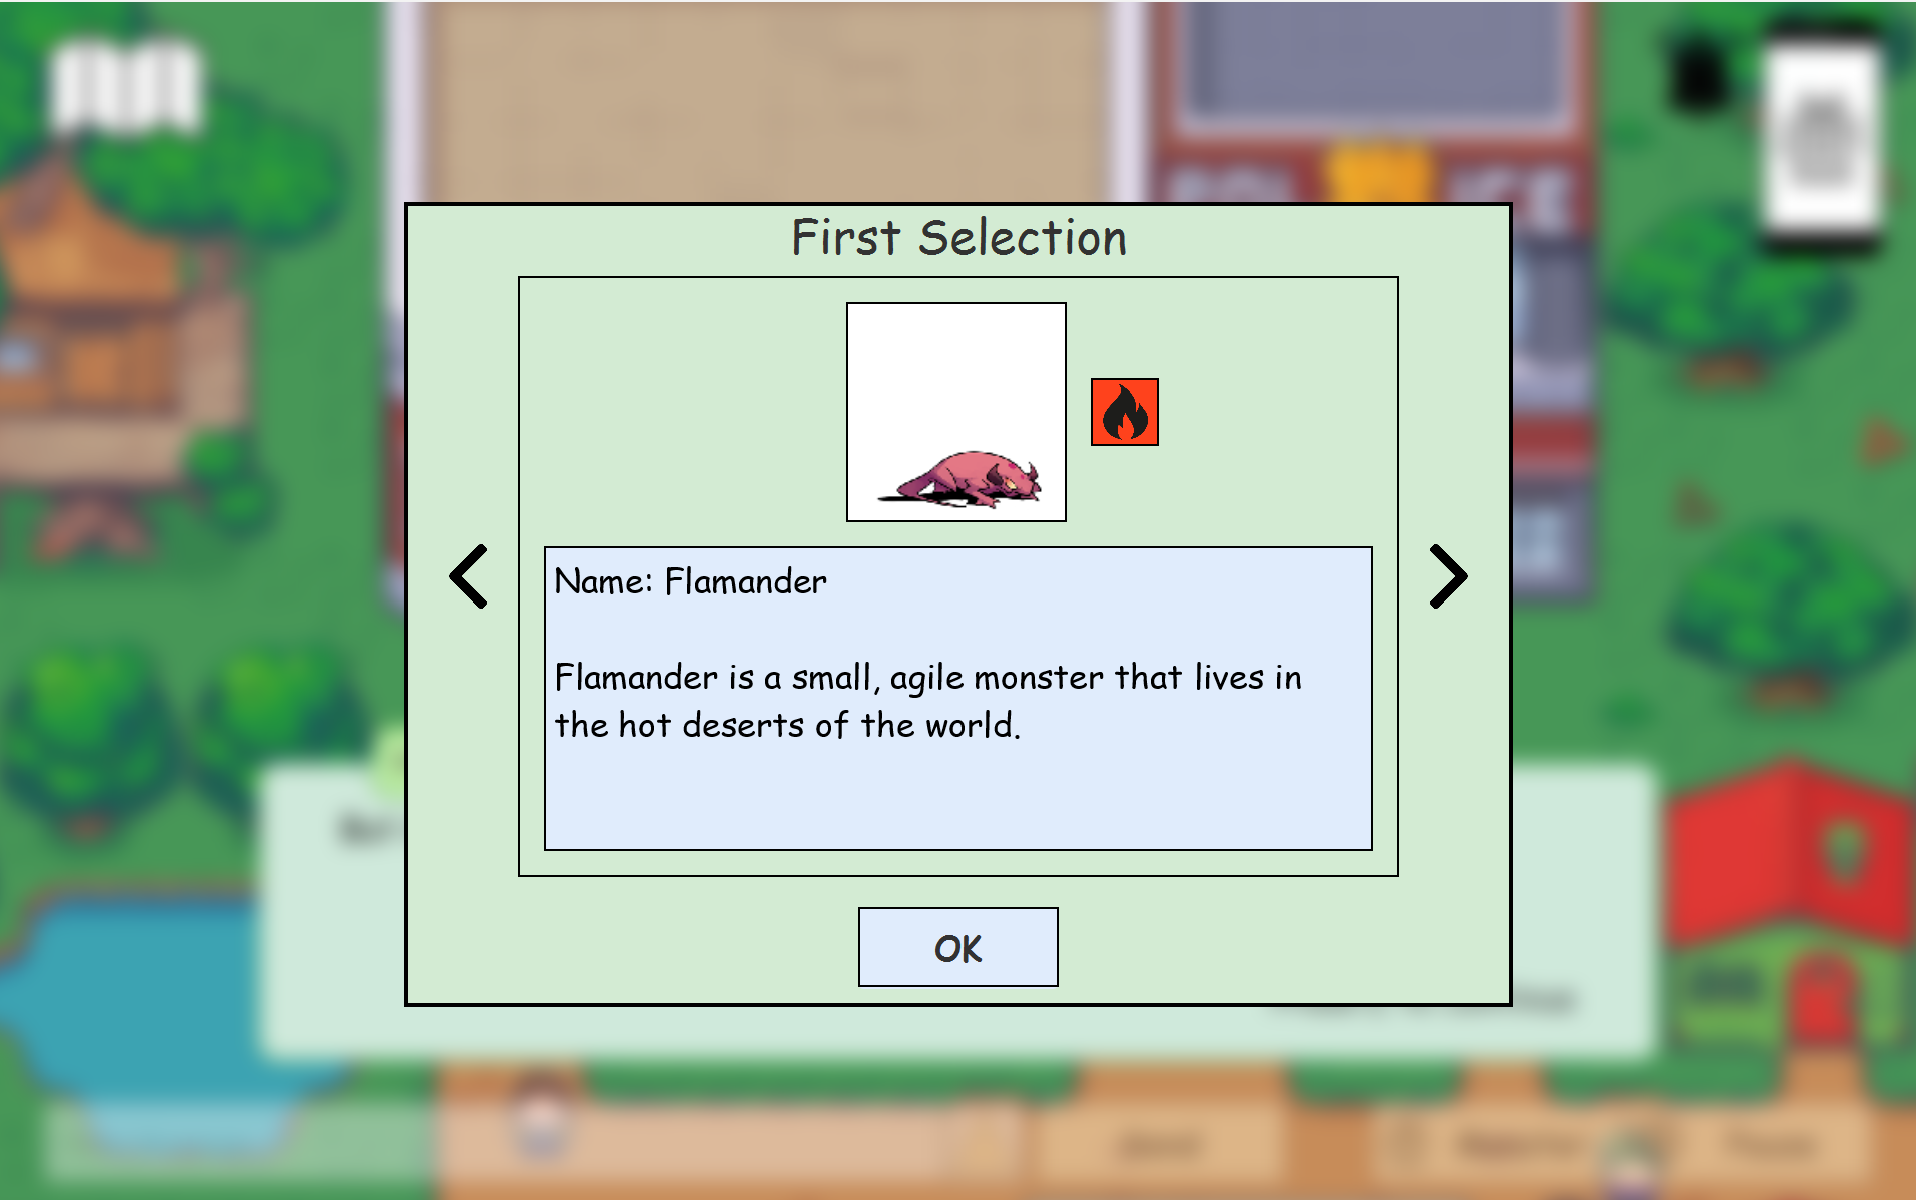
\includegraphics[width=\textwidth]{images/implementation/Starter/Starter selection implementation.png}
        \caption{Implementierung: Erste Auswahl an Starter-Monstern}
        \label{fig: Implementierung: Erste Auswahl an Starter-Monstern}
    \end{subfigure}
    \caption{Vergleich: Auswahl an Starter-Monsters}
    \label{fig: Vergleich: Auswahl an Starter-Monsters}
\end{figure}
\begin{figure}[H]
    \centering
    \begin{subfigure}[b]{0.4\textwidth}
        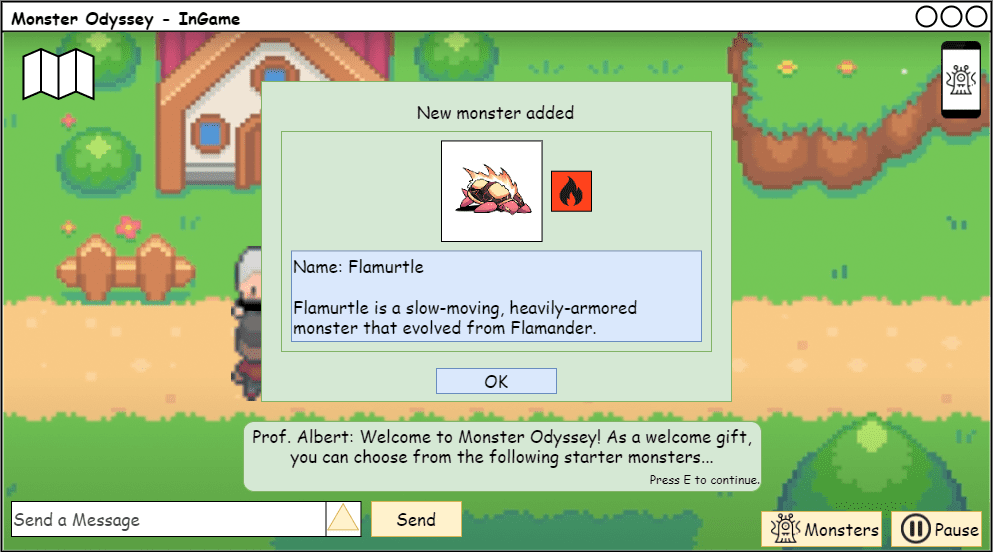
\includegraphics[width=\textwidth]{images/mockups/Starter/PlayerAndProfMonsterReceived}
        \caption{Mockup: Erhalt des Starter-Monsters}
        \label{fig: Mockup: Erhaltener Starter-Monster}
    \end{subfigure}
    \hfill
    \begin{subfigure}[b]{0.4\textwidth}
        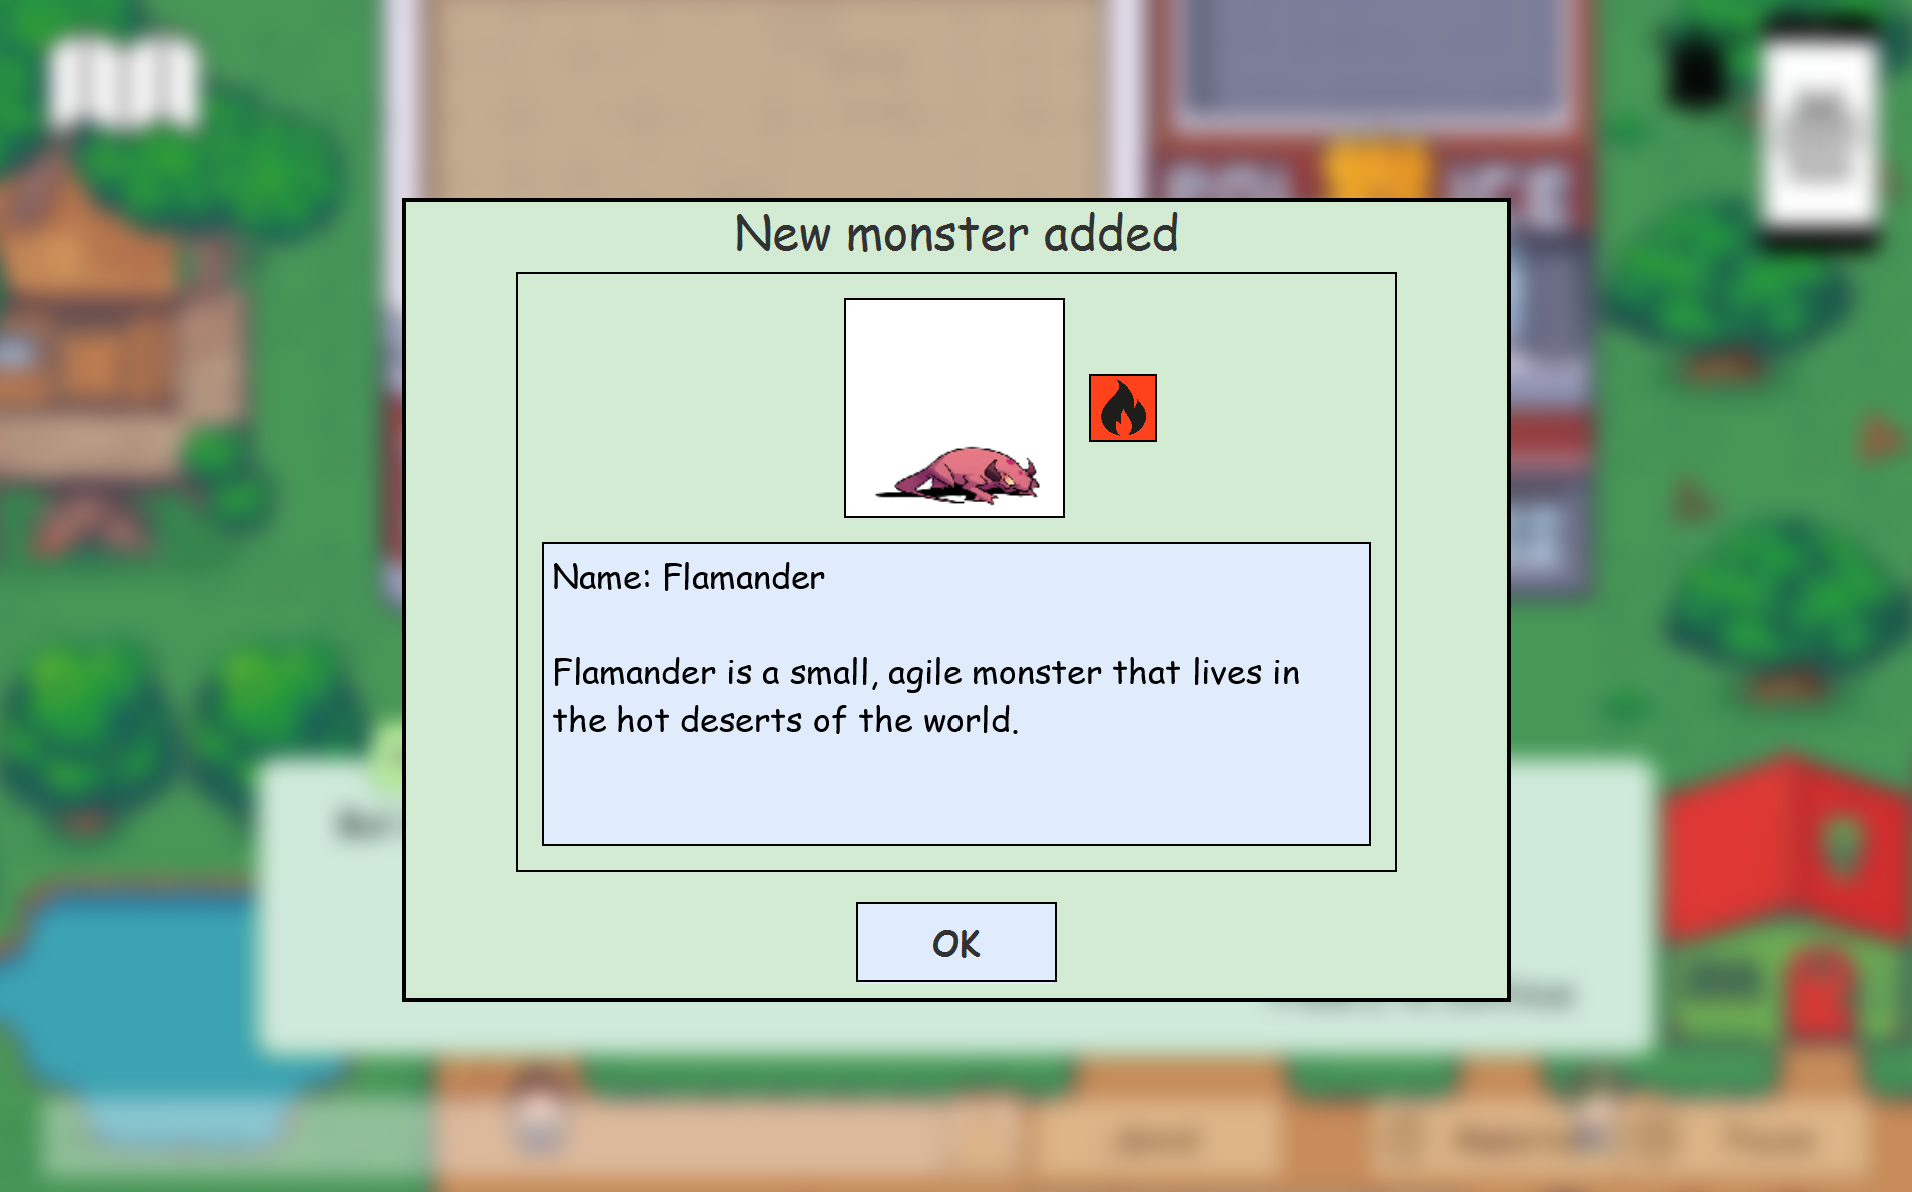
\includegraphics[width=\textwidth]{images/implementation/Starter/New Monster added implementation.png}
        \caption{Implementierung: Erhalt des Starter-Monsters}
        \label{fig: Implementierung: Erhaltener Starter-Monster}
    \end{subfigure}
    \caption{Vergleich: Erhalt des Starter-Monsters}
    \label{fig: Vergleich: Erhaltener Starter-Monster}
\end{figure}